\documentclass{article}\usepackage[]{graphicx}\usepackage[]{color}
%% maxwidth is the original width if it is less than linewidth
%% otherwise use linewidth (to make sure the graphics do not exceed the margin)
\makeatletter
\def\maxwidth{ %
  \ifdim\Gin@nat@width>\linewidth
    \linewidth
  \else
    \Gin@nat@width
  \fi
}
\makeatother

\definecolor{fgcolor}{rgb}{0.345, 0.345, 0.345}
\newcommand{\hlnum}[1]{\textcolor[rgb]{0.686,0.059,0.569}{#1}}%
\newcommand{\hlstr}[1]{\textcolor[rgb]{0.192,0.494,0.8}{#1}}%
\newcommand{\hlcom}[1]{\textcolor[rgb]{0.678,0.584,0.686}{\textit{#1}}}%
\newcommand{\hlopt}[1]{\textcolor[rgb]{0,0,0}{#1}}%
\newcommand{\hlstd}[1]{\textcolor[rgb]{0.345,0.345,0.345}{#1}}%
\newcommand{\hlkwa}[1]{\textcolor[rgb]{0.161,0.373,0.58}{\textbf{#1}}}%
\newcommand{\hlkwb}[1]{\textcolor[rgb]{0.69,0.353,0.396}{#1}}%
\newcommand{\hlkwc}[1]{\textcolor[rgb]{0.333,0.667,0.333}{#1}}%
\newcommand{\hlkwd}[1]{\textcolor[rgb]{0.737,0.353,0.396}{\textbf{#1}}}%

\usepackage{framed}
\makeatletter
\newenvironment{kframe}{%
 \def\at@end@of@kframe{}%
 \ifinner\ifhmode%
  \def\at@end@of@kframe{\end{minipage}}%
  \begin{minipage}{\columnwidth}%
 \fi\fi%
 \def\FrameCommand##1{\hskip\@totalleftmargin \hskip-\fboxsep
 \colorbox{shadecolor}{##1}\hskip-\fboxsep
     % There is no \\@totalrightmargin, so:
     \hskip-\linewidth \hskip-\@totalleftmargin \hskip\columnwidth}%
 \MakeFramed {\advance\hsize-\width
   \@totalleftmargin\z@ \linewidth\hsize
   \@setminipage}}%
 {\par\unskip\endMakeFramed%
 \at@end@of@kframe}
\makeatother

\definecolor{shadecolor}{rgb}{.97, .97, .97}
\definecolor{messagecolor}{rgb}{0, 0, 0}
\definecolor{warningcolor}{rgb}{1, 0, 1}
\definecolor{errorcolor}{rgb}{1, 0, 0}
\newenvironment{knitrout}{}{} % an empty environment to be redefined in TeX

\usepackage{alltt}
\usepackage{Sweave}
\usepackage{graphicx}
\usepackage{tabularx}
\usepackage[small]{caption}
\usepackage{gensymb}
\usepackage{float}
\usepackage{subfig}
\usepackage{url}
\setkeys{Gin}{width=0.8\textwidth}
\setlength{\captionmargin}{30pt}
\setlength{\abovecaptionskip}{0pt}
\setlength{\belowcaptionskip}{10pt}
\topmargin -1.5cm        
\oddsidemargin -0.04cm   
\evensidemargin -0.04cm
\textwidth 16.59cm
\textheight 21.94cm 
\pagestyle{empty}
\parskip 7.2pt
\renewcommand{\baselinestretch}{1.5}
\parindent 0pt
\IfFileExists{upquote.sty}{\usepackage{upquote}}{}
\begin{document}

\renewcommand{\thetable}{\arabic{table}}
\renewcommand{\thefigure}{\arabic{figure}}
\renewcommand{\labelitemi}{$-$}
%%%%%%%%%%%%%%%%%%%%%%%%%%%%%%%%%%%%%%%%%%%%%%%%%%%%%%%
\begin{center}
{\huge\textbf{Pignut Hickory - {\textit{Carya glabra}}}}
\end{center}
\section*{Overview}
The pignut hickory is part of the Walnut family, or the Juglandaceae family. It is a medium to large sized tree, roughly 60-80 feet tall (18-24m) and has a trunk diameter of 1-2 feet (0.3-0.6m). The canopy width is generally 25-40 feet (7-12m). The pignut hickory typically grows in dry and moist uplands in hardwood forests in communities of oaks and other hickory trees and blooms around April or May. 
\section*{Habitat and Growth}
The pignut hickory grows best in rich, medium moisture soil that is well-drained and in an area that receives full to partial sun. The tree requires a lot of space to grow and is difficult to transplant due to its pronounced taproot and few lateral roots. It is commonly found on ridges or hillslopes and is most prevalent along the Appalachian forests and the lower Ohio River Basin. The pignut hickory does not have any serious insect or disease problems, however the hickory bark beetle, weevils,  and borers can occassionally cause damage in certain regions of the range. The pignut hickory is not known as an ornamental tree but it is commonly planted within large properties or parks for shade. The range can be seen in Figure 1. Given the wide range and distribution of the species, it can grow in temperatures ranging from -30\degree{C} to 46\degree{C} (-22 to 115\degree{F}). Although the growing season will vary by latitude and elevation. Pignut hickories are a common species but not generally abundant. They are often found in upland climax forests alongside other hickory species and oak species. 
\begin{figure}[ht]
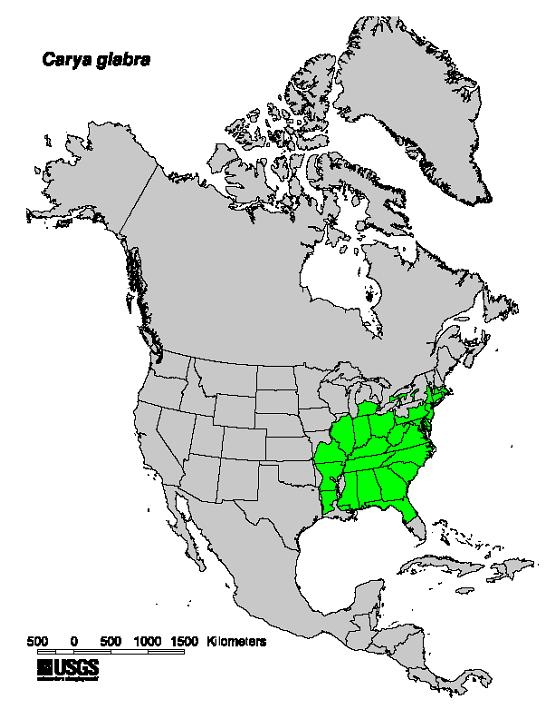
\includegraphics[width=0.5\textwidth]{Carya_glabra_range_map.jpg}
\centering
\caption{Distribution map of \textit{Carya glabra} throughout North America}
\end{figure}
\newpage
\subsection*{Description}
Pignut hickory leaves are alternate, pinnately compound with a terminal leaflet that is typically longer than the lateral leaflets. Leaves generally have 5-7 leaflets -- rarely 3 -- and are mostly hairless. The base is wedge-shaped and the tip narrows to a point. Leaf margins are sharply or coarsely toothed. The upper surface of the leaflets are a darker green and completely hairless, whereas the lower surface is a paler green and usually hairless but can have small tufts of hair along the veins. The bark is gray and tightly furrowed and pignut hickories have a single, straight trunk. 
\begin{figure}[ht]%
    \centering
    \subfloat[Pignut Hickory Budbreak]{{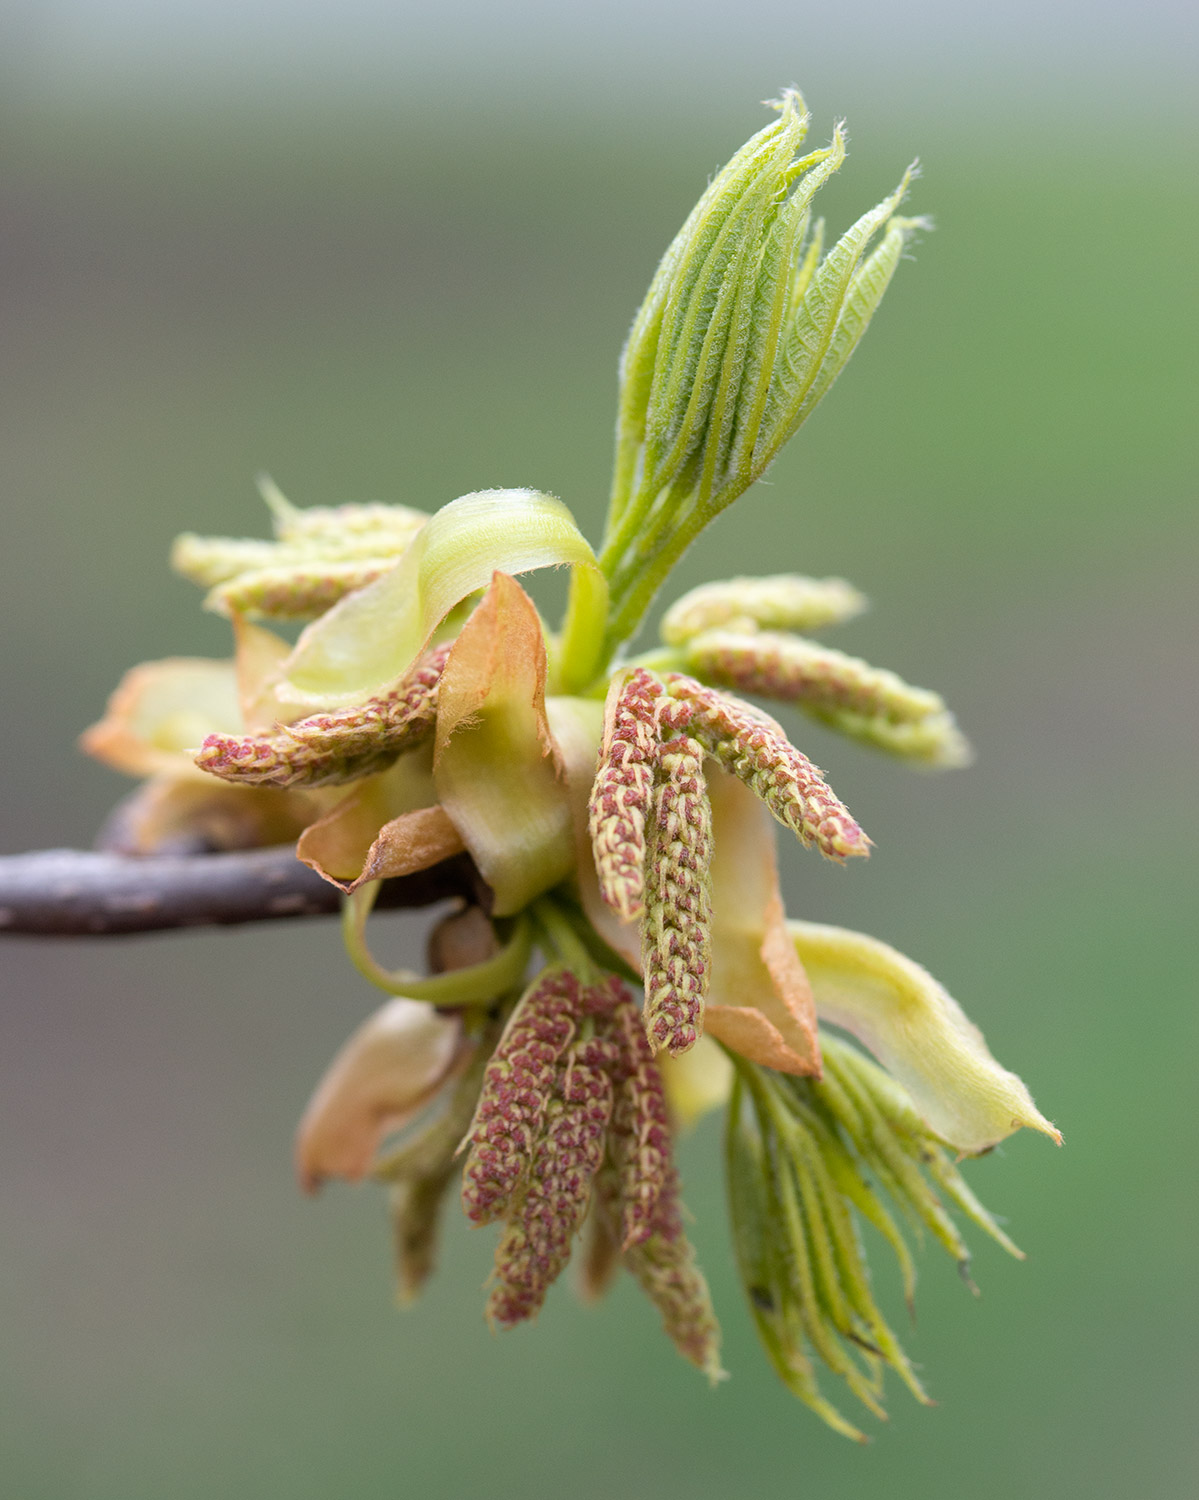
\includegraphics[width=7cm]{pignut_budbreak.jpg} }}%
    \qquad
    \subfloat[Pignut Hickory Juvenile Leaves]{{\includegraphics[width=7cm]{pignut_leaves.jpg} }}%
    \caption{Pignut Hickory Budbreak and Increasing Leaf Size}%
    \label{fig:leaves}%
\end{figure}
\newpage
\subsection*{Reproduction and Propogation}
Pignut hickories are monoecious. Flowers open starting from the middle of March in the southeast to early June around the northeastern region of the range. This tree reaches maturity around 30 years of age, which is when flowering begins. Male catkins are found in drooping clusters at the tips of young twigs and are typically yellow-green in color. The female flowers are shorter and grow in groups of one to five spikes. They are also generally greener in color. Optimal seed production usually takes place between 75 to 200 years of age but can extend through 300 years of age. Pignut hickories have the lightest seed of the hickory species, about there are about 200/lb. Dissemination is through gravity, however, squirrels and chipmunks can aid the process. Late spring frosts can greatly hinder seed production. The fruit is pear shaped and enclosed in a thin husk (Figure 3a). It ripens around September and October (Figure 3b) and seeds are dispered from September through December. Fruits are green until they reach maturity, when they turn a brownish color. 
\begin{figure}[ht]%
    \centering
    \subfloat[Pignut Hickory Fruit]{{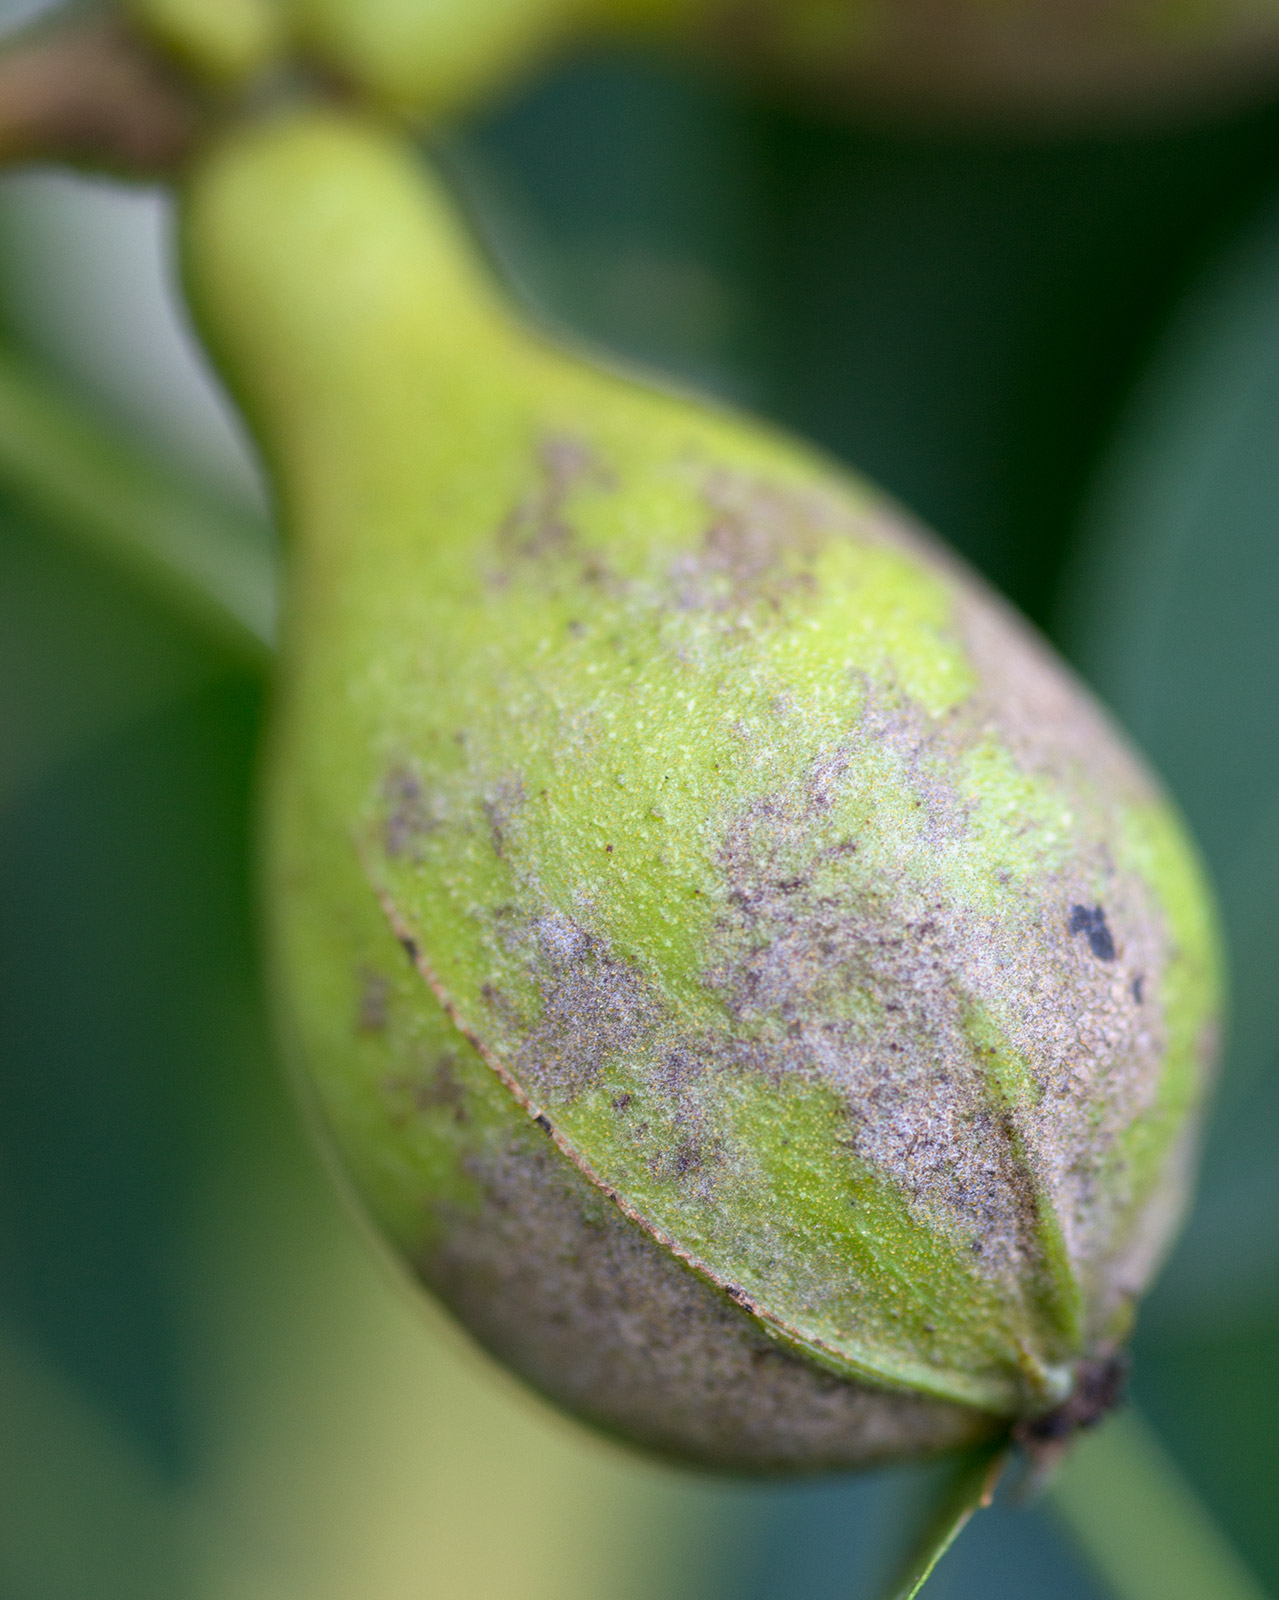
\includegraphics[width=7cm]{pignut_fruit.jpg} }}%
    \qquad
    \subfloat[Ripe Pignut Hickory Fruit]{{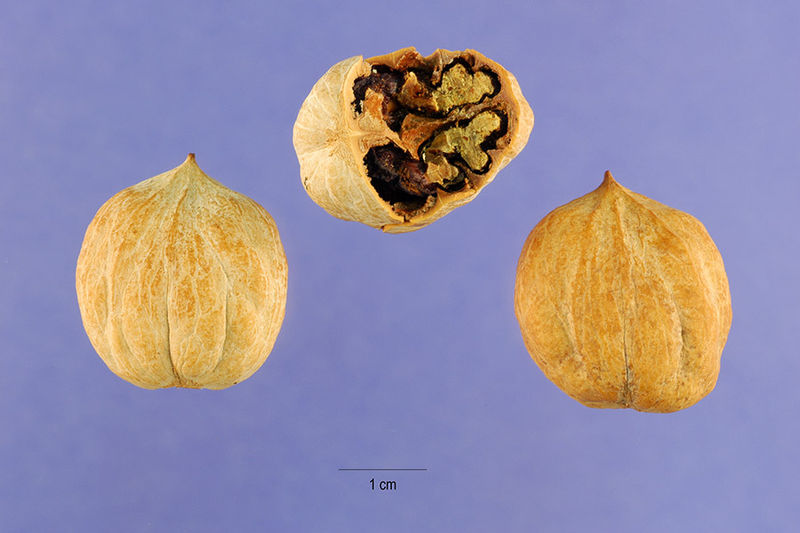
\includegraphics[width=7cm]{ripe_pignut.jpg} }}%
    \caption{Pignut Hickor Fruit Phenophases}%
    \label{fig:fruit}%
\end{figure}
\newpage
\section*{Relation to other Hickories}
Surprisingly, the Pignut Hickory is most closely related to the Sand Hickory with the only distinguishing feature being the hairy petiole and rachis of the leaf on the Sand Hickory. The Pignut Hickory is still very similar to the Shagbark Hickory, except the pignut can have 5-7 leaflets where the shagbark only has 5. The fruits are slightly more pear shaped on the pignut and the leaves are nearly hairless on the pignut than the shagbark. The greatest distinctive feature, however, is the bark. The shagbark has a very distinct shaggy bark (Figure 4a), while the pignut is moderately to tightly furrowed (Figure 4b). 
\\
{\textbf{Interesting Facts:}}
There are three groups of hickory trees: pecans, shagbarks, and pignuts. There are four pecan species, three shagbark species, and four pignut species. The pignuts are distinguished from the pecans and shagbarks by their tightly furrowed bark, slender twigs, thinner fruit husks, and smaller leaf buds. The seedlings do not tolerate shade very well, in comparison to the shagbark, which is a much hardier species. 
\begin{figure}[ht]%
    \centering
    \subfloat[Pignut Hickory Bark]{{\includegraphics[width=7cm]{pignut_bark.jpg} }}%
    \qquad
    \subfloat[Shagbark Hickory Bark]{{\includegraphics[width=7cm]{shagbark_bark.jpg} }}%
    \caption{Comparison of bark between the Pignut and Shagbark hickory species}%
    \label{fig:bark}%
\end{figure}
\newpage
\section*{Why Study this Species?}
One of the primary reasons for the NPN choosing this species is due to its range. It is pretty locally distributed, mainly growing along the East coast. By analyzing the phenological changes of the pignut hickory, the NPN can pool its data and compare the differences in plant responses across the various geographical regions in the US. Like the other trees, it is also an allergen, so understanding the phenophases helps alert the public when allergen risks are higher. The NPN is also asking for volunteers to take note if there is evidence of leaf color change due to drought by making a notation in the comments section of the datasheets. 
\newpage
\section*{References}
\url{http://dendro.cnre.vt.edu/dendrology/syllabus/factsheet.cfm?ID=19} \\
\url{http://plants.usda.gov/core/profile?symbol=cagl8} \\
\url{http://www.missouribotanicalgarden.org/PlantFinder/PlantFinderDetails.aspx?kempercode=d376} \\
\url{https://www.na.fs.fed.us/pubs/silvics_manual/volume_2/carya/glabra.htm} \\
\url{https://www.usanpn.org/nn/Carya_glabra}\\
\url{http://caseytrees.org/tree-species/pignut-hickory/}\\
\url{http://www.museum.state.il.us/muslink/forest/htmls/trees/C-glabra.html}

\end{document}
